% "{'classe':('PSI','MP'),'chapitre':'slci_revisions','type':(''),'titre':'Exosquelette lombaire', 'source':'Concours Centrale-Supélec 2023','comp':(None),'corrige':True}"
%\setchapterimage{bandeau}
\chapter*{TD \arabic{cptTD} \\ 
Exosquelette lombaire -- 
\ifprof Corrigé \else Sujet \fi}
\addcontentsline{toc}{section}{TD \arabic{cptTD} :
Exosquelette lombaire -- 
\ifprof Corrigé \else Sujet \fi}

\iflivret \stepcounter{cptTD} \else
\ifprof  \stepcounter{cptTD} \else \fi
\fi

\setcounter{question}{0}
\marginnote{Concours Centrale-Supélec 2023 -- MP.}
%\marginnote[1cm]{
%\UPSTIcompetence[2]{C1-02}
%\UPSTIcompetence[2]{C2-04}}

\begin{marginfigure}
\centering
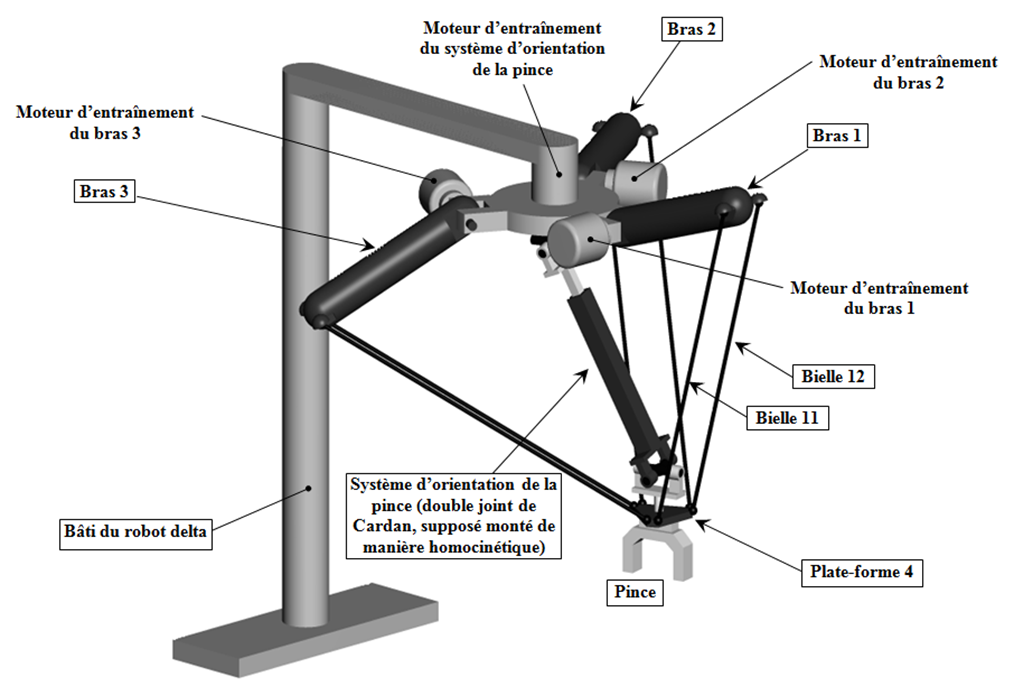
\includegraphics[width=\linewidth]{fig_01}
\caption{Exosquelette lombaire Japet \label{Cy_02_Ch_04_TD_02_fig_01}}
\end{marginfigure}

\subsection*{Mise en situation}
\ifprof
\else
On s'intéresse à un banc d'essai permettant de valider un actionneur linéaire. 
Dans ce cadre, il est nécessaire de proposer un modèle de connaissance de l’asservissement en force, le valider par comparaison avec une mesure sur le banc d’essai et vérifier les performances de l’actionneur linéaire sur ce banc d’essai. Ce modèle permettra de valider une commande pour le cas spécifique étudié.

Le schéma-blocs est donné dans la figure \ref{Cy_02_Ch_04_TD_02_fig_11}.

\begin{figure*}[!h]
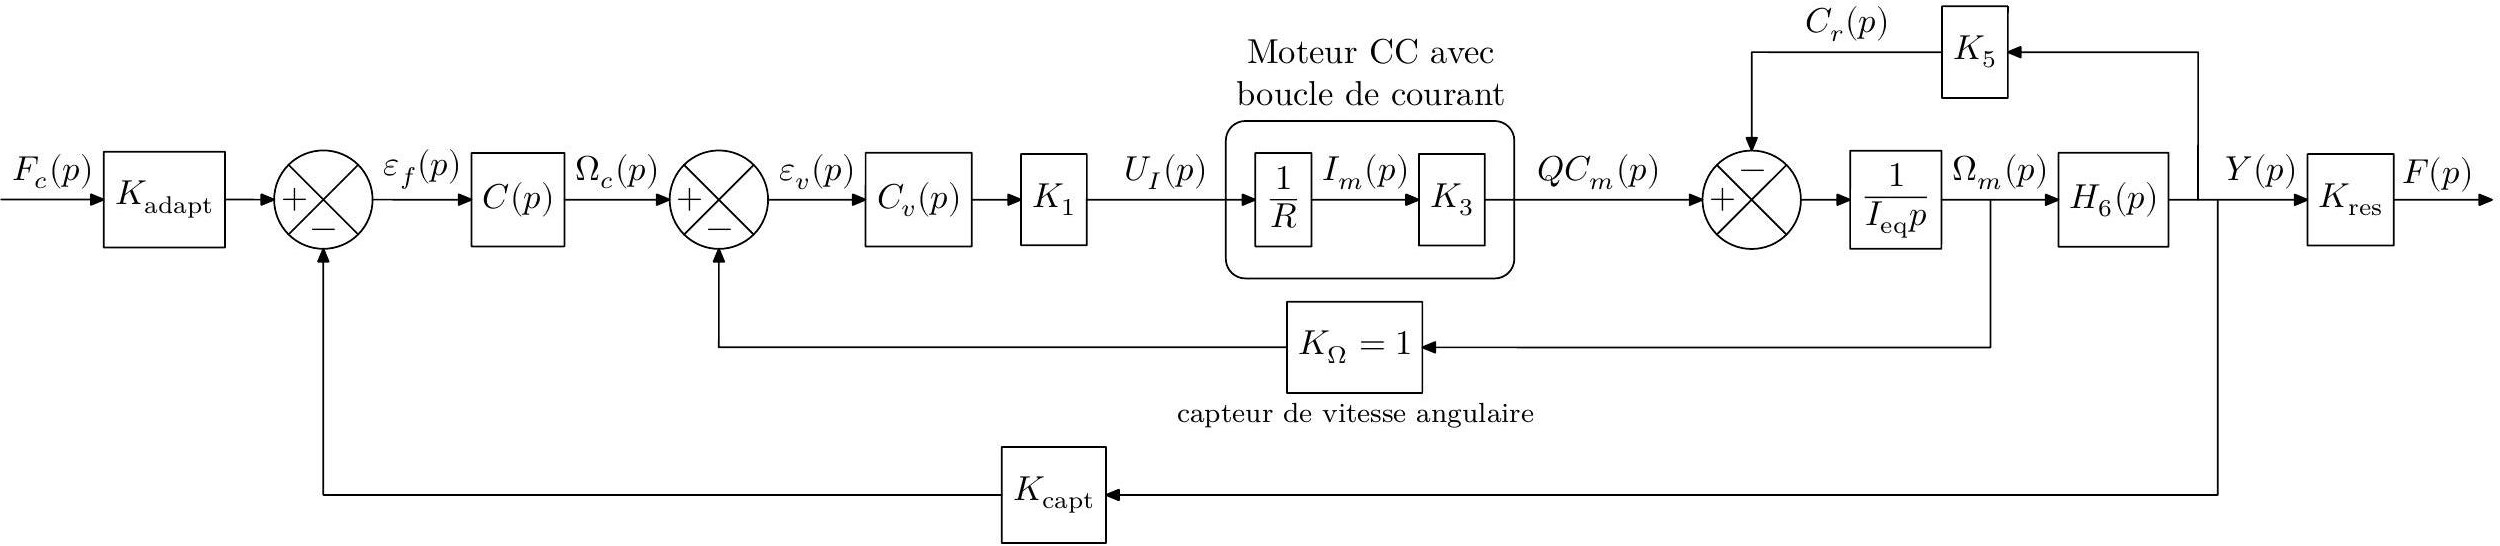
\includegraphics[width=\linewidth]{2024_03_20_0c3cf888f6e04b1986bcg-09}
\caption{ Schéma-blocs de l’asservissement de force
 développée par un actionneur linéaire placé sur le banc d’essai \label{Cy_02_Ch_04_TD_02_fig_11}}
\end{figure*}

\fi


\subsection*{Réglage de la boucle d'asservissement de la vitesse angulaire du moteur}

\ifprof
\else
Le schéma-blocs décrivant la structure de l'asservissement de la vitesse angulaire du moteur est fourni sur la figure \ref{Cy_02_Ch_04_TD_02_fig_12}. Cet asservissement doit respecter le cahier des charges fourni dans le tableau \ref{Cy_02_Ch_04_TD_02_tab_04}.

\begin{figure}[!h]
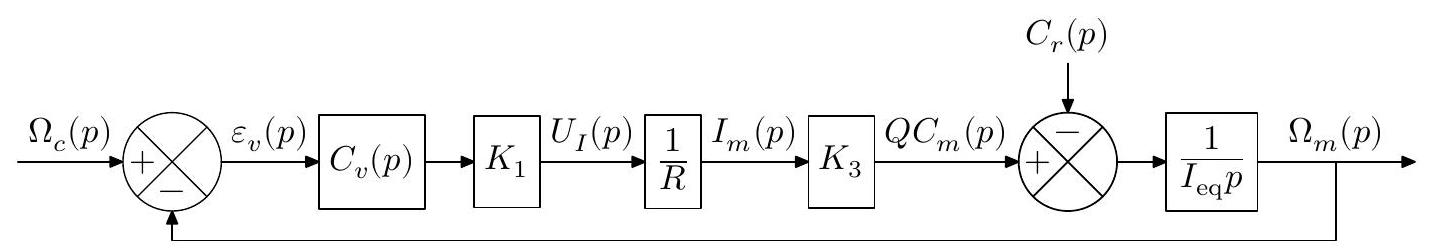
\includegraphics[width=\textwidth]{2024_03_20_0c3cf888f6e04b1986bcg-10}
\caption{Schéma-blocs de la boucle d'asservissement de la vitesse angulaire du moteur électrique \label{Cy_02_Ch_04_TD_02_fig_12}}
\end{figure}

\begin{table}[!h]
\begin{tabular}{p{9cm}l}
\hline
\textbf{Critère concepteur} & \textbf{Niveau} \\
\hline
Marge de phase & $\geqslant 80^{\circ}$ \\
Erreur en régime permanent pour une perturbation en échelon constante & Nulle \\
Pulsation de coupure à $0 \mathrm{~dB}$ & $\omega_{0 \mathrm{~dB}}=10 \mathrm{rad} \cdot \mathrm{s}^{-1}$ \\
\hline
\end{tabular}
\caption{Critères concepteur pour la boucle d'asservissement de la vitesse angulaire \label{Cy_02_Ch_04_TD_02_tab_04}}
\end{table}

Le choix d'un correcteur proportionnel intégral est fait afin de diminuer l'influence de la perturbation en couple modélisée par $C_{r}(p)$. La fonction de transfert du correcteur de la boucle d'asservissement en vitesse angulaire est noté $C_{v}(p)$, tel que $C_{v}(p)=K_{i} \frac{1+\tau_{i} p}{\tau_{i} p}$.


On note $\indice{H}{BOv}(p)=\frac{\Omega_{m}(p)}{\varepsilon_{v}(p)}$ la fonction de transfert en boucle ouverte de l'asservissement de vitesse angulaire du moteur.

\fi

%Q 17. 
\question{Déterminer l'expression littérale de la phase de $\indice{H}{BOv}(\mathrm{i} \omega)$. En déduire la valeur numérique de $\tau_{i}$ respectant les critères concepteur de la boucle de vitesse. \label{Cy_02_Ch_04_TD_02_q_17}}
\ifprof
\begin{corrige}
On a $\indice{H}{BOv}(\mathrm{i} \omega) = C_v(p)K_1 \dfrac{1}{R}K_3 \dfrac{1}{\indice{I}{eq}p}$
$= \dfrac{K_{i} K_1 K_3 }{R \indice{I}{eq}}  \frac{1+\tau_{i} p}{\tau_{i} p^2} $.

On a $\varphi(\omega)=\arg\left({\dfrac{K_{i} K_1 K_3 }{R \indice{I}{eq}}}\right) + \arg\left( 1+\tau_{i} p\right) - \arg\left( \tau_{i} p^2\right) $ $=\arctan{\tau_i \omega } - 180\degres$.

On souhaite une marge de phase supérieure à 80\degres; donc $M_{\varphi} = \varphi(\omega) + 180$  $=\arctan{\tau_i \omega} \geq 80\degres$.

$\arctan{\tau_i \omega} \geq 80\degres$ 
$\Rightarrow  \tau_i \omega \geq \tan 80$
$\Rightarrow  \tau_i  \geq \dfrac{\tan 80}{\omega_{\SI{0}{dB}}}$
$\Rightarrow  \tau_i  \geq \SI{0,57}{s}$.
\end{corrige}
\else
\fi

\ifprof
\else
Le diagramme de Bode de la boucle ouverte $H_{B O v}(p)$, avec $K_{i}=1$ et $\tau_{i}$ déterminé à la question \ref{Cy_02_Ch_04_TD_02_q_17} , est donné sur la figure \ref{Cy_02_Ch_04_TD_02_fig_13}.



\begin{figure}[!h]
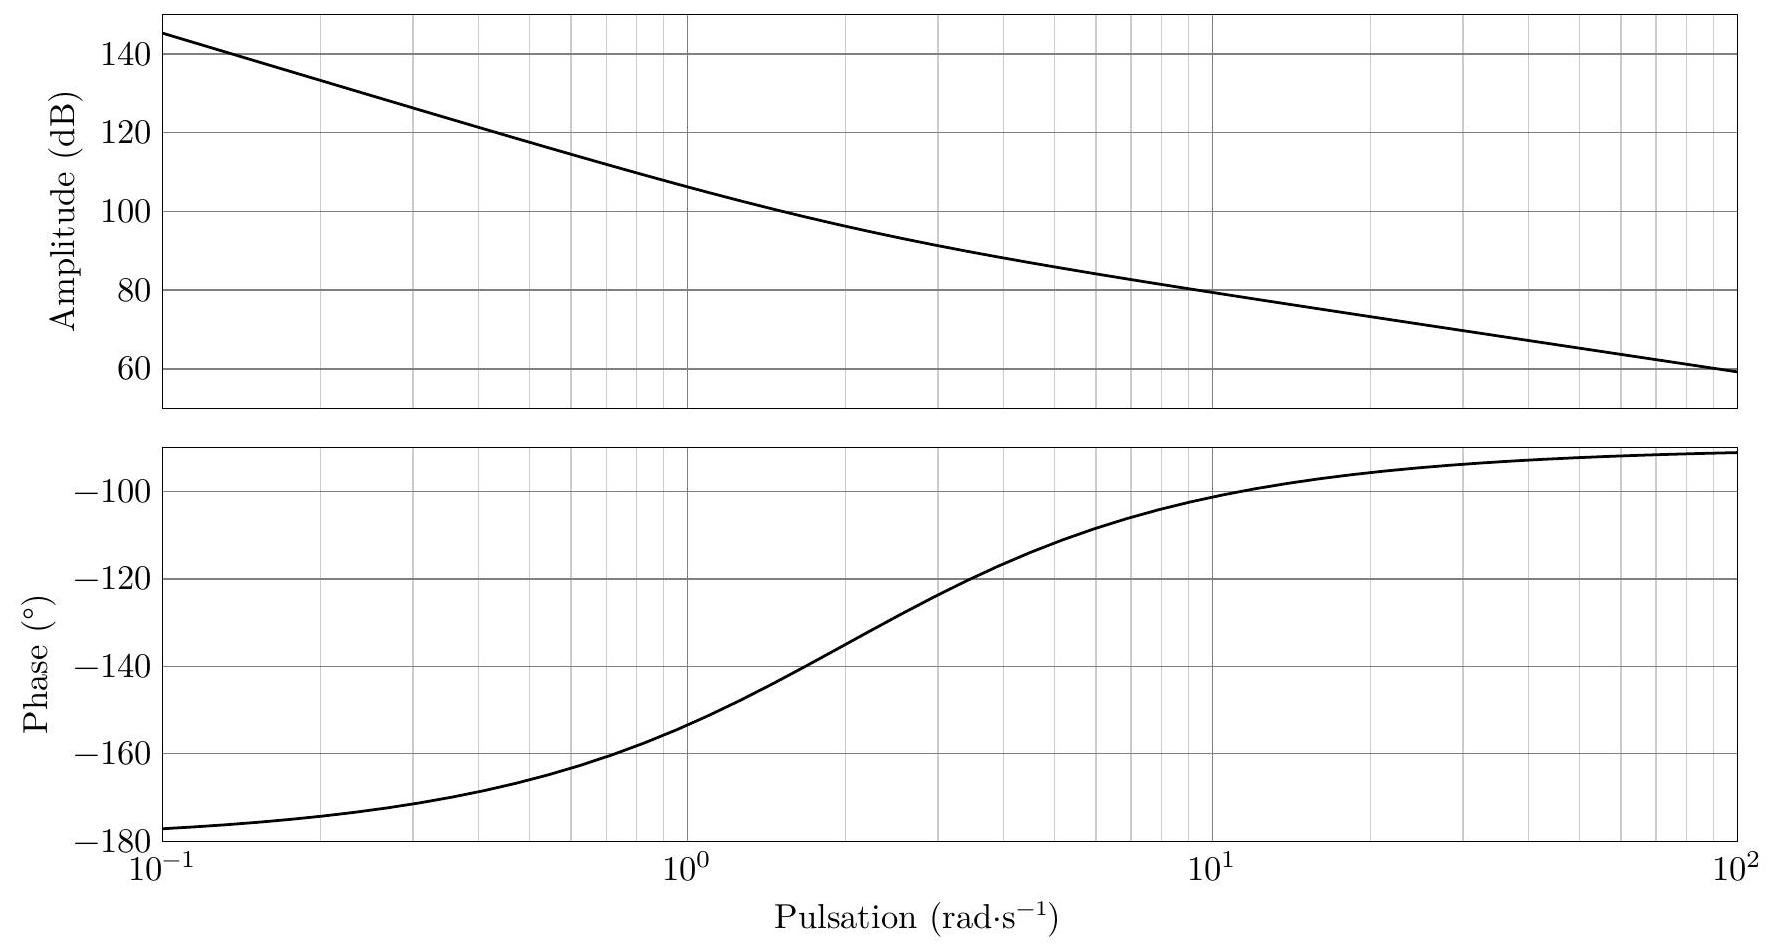
\includegraphics[width=\textwidth]{2024_03_20_0c3cf888f6e04b1986bcg-10(1)}
\caption{Diagramme de Bode de $\indice{H}{BOv}(p)$ \label{Cy_02_Ch_04_TD_02_fig_13}}
\end{figure}
\fi


%Q 18. 
\question{Déterminer la valeur numérique de $K_{i}$ afin que la boucle d'asservissement de vitesse respecte les critères concepteur du tableau \ref{Cy_02_Ch_04_TD_02_tab_04}. \label{Cy_02_Ch_04_TD_02_q_18}}
\ifprof
\begin{corrige}
Pour $\omega_{\SI{0}{dB}}=\SI{10}{rad.s^{-1}}$ on mesure un gain de \SI{80}{dB}. 
Il faut donc déterminer $K_i$ tel que $20\log K_i = -80$ soit $K_i = \SI{1e{-4}}{V.s.rad^{-1}} $. 


Les critères de marge et de pulsation de coupure sont respectés (on a tout fait pour).
L'erreur statique est nulle car il y a un intégarteur dans le correcteur (elle sera nulle à condition que la perturbation soit constante).

\end{corrige}
\else
\fi

\subsection*{Simplification du modèle de connaissance}
\ifprof
\else
Il est possible de mettre le schéma-blocs de la figure \ref{Cy_02_Ch_04_TD_02_fig_11} 
sous la forme du schéma-blocs de la figure \ref{Cy_02_Ch_04_TD_02_fig_14}, afin de faciliter la prévision des performances simulées.

\begin{figure}[!h]
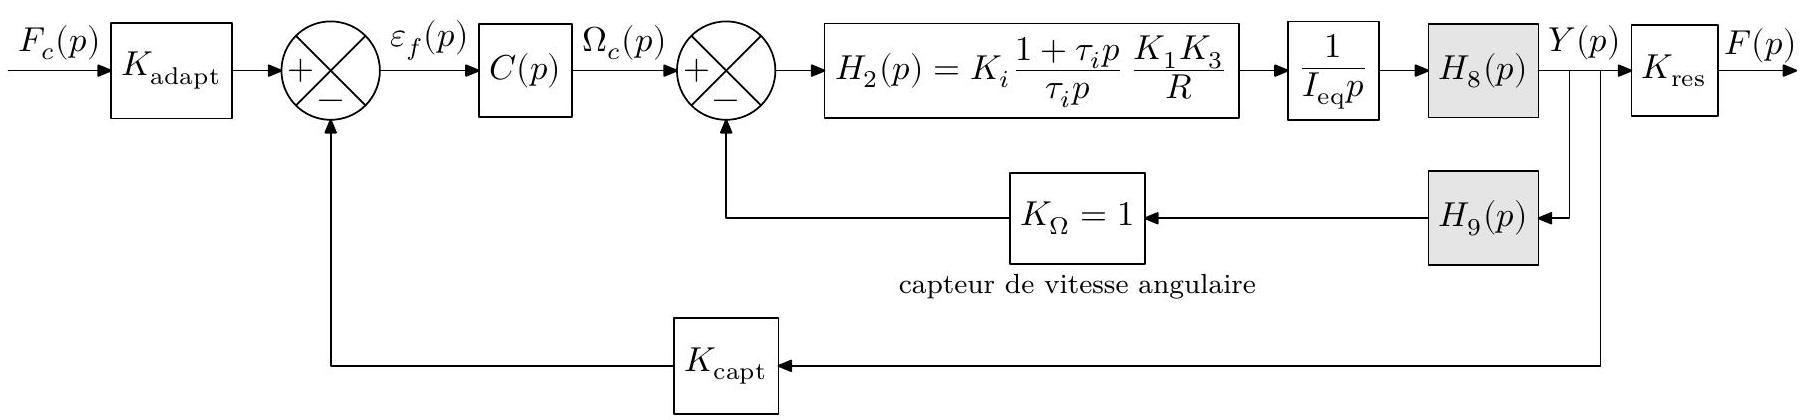
\includegraphics[width=\textwidth]{2024_03_20_0c3cf888f6e04b1986bcg-11(1)}
\caption{Schéma-blocs de l'asservissement de la force développée par un actionneur linéaire \label{Cy_02_Ch_04_TD_02_fig_14}}
\end{figure}
\fi

%Q 19
\question{Déterminer les fonctions de transfert $H_{8}(p)$ et $H_{9}(p)$ en fonction de $K_{5}, I_{\text {eq}}$ et $H_{6}(p)$. Ne pas remplacer $K_{5}$ et $H_{6}(p)$ par les expressions trouvées précédemment. \label{Cy_02_Ch_04_TD_02_q_19}}
\ifprof
\begin{corrige}
En décalant le point de prélèvement du capteur de vitesse d'un bloc vers la droite, on se retrouve avec $\dfrac{1}{H_6(p)}$ dans la boucle de retour. 

On sort le bloc $\dfrac{1}{\indice{I}{eq}p}$ de la << petite >> boucle et $\dfrac{1}{\indice{I}{eq}p}$ se retrouve aussi dans la pboucle de retour. 

En identifiant, on a alors $H_9(p)=\dfrac{1}{H_6(p)}$ et en utilisant la formule de Black, on a 
$H_8(p)=\dfrac{H_6(p)}{1+ \dfrac{H_6(p) K_5}{\indice{I}{eq}p} }$ $=\dfrac{H_6(p) \indice{I}{eq}p}{\indice{I}{eq}p+H_6(p) K_5 }$.


\end{corrige}
\else
\fi

\ifprof
\else
Pour faciliter l'analyse des performances simulées, le schéma-blocs de la figure \ref{Cy_02_Ch_04_TD_02_fig_14} est adapté afin de disposer d'un schéma-blocs 
à retour unitaire, tel que décrit sur la figure \ref{Cy_02_Ch_04_TD_02_fig_15}.


\begin{figure}[!h]
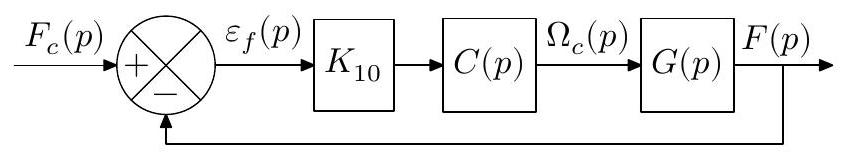
\includegraphics[width=.6\textwidth]{2024_03_20_0c3cf888f6e04b1986bcg-11}
\caption{Schéma-blocs de l'asservissement de la force développée par un actionneur linéaire à retour unitaire \label{Cy_02_Ch_04_TD_02_fig_15}}
\end{figure}
\fi


%Q 20
\question{Déterminer l'expression du gain $K_{10}$ en fonction de $K_{\text{capt}}$ 
et de $K_{\text{res}}$. \label{Cy_02_Ch_04_TD_02_q_20}}
\ifprof
\begin{corrige}
En décalant le point de prélèvement de droite vers la droite, on a alors $\indice{K}{res}$ dans la boucle de retour. 
Pour que le système soit correctement asservi, il faut donc nécessairement que 
$\indice{K}{adapt} = \indice{K}{capt}\indice{K}{res}$

On se ramène ensuite à un retour unitaire. On alors $\indice{K}{10} = \indice{K}{capt}\indice{K}{res}$.
\end{corrige}
\else
\fi

%Q 21
\question{Déterminer la fonction de transfert $G(p)$ en fonction de $H_{2}(p), I_{\text {eq}}, H_{8}(p),  H_{9}(p)$ et $K_{\text {res }}$. Ne pas remplacer $H_{2}(p), H_{8}(p)$ et $H_{9}(p)$ par les expressions trouvées précédemment. \label{Cy_02_Ch_04_TD_02_q_21}}
\ifprof
\begin{corrige}
$G(p)=\dfrac{H_2(p)\dfrac{1}{\indice{J}{eq}p}H_8(p)}{1+H_2(p)H_8(p)H_9(p)\dfrac{1}{\indice{J}{eq}p}}\indice{K}{res}$
$ = \dfrac{H_2(p)H_8(p)}{\indice{J}{eq}p+H_2(p)H_8(p)H_9(p)}\indice{K}{res}$
\end{corrige}
\else
\fi

Pour la suite, on donne la fonction de transfert $G(p)$, obtenue avec les valeurs de réglage correctes déterminées aux questions \ref{Cy_02_Ch_04_TD_02_q_17} et \ref{Cy_02_Ch_04_TD_02_q_18},

$$
G(p)=\frac{F(p)}{\Omega_{c}(p)}=\frac{1+\tau_{i} p}{p} \frac{1,2 \times 10^{-5}}{2 \times 10^{-4}+9,7 \times 10^{-5} p+5,3 \times 10^{-6} p^{2}} .
$$

\subsection*{Analyse des performances de l'asservissement en force développée par un actionneur linéaire}
\ifprof
\else
Il est proposé dans cette section d'analyser les performances simulées de l'asservissement en force dont un extrait du cahier des charges est présenté dans le tableau~\ref{Cy_02_Ch_04_TD_02_tab_05}.

\begin{table}[!h]
\begin{tabular}{llp{7cm}l}
\hline
\textbf{Id} & \textbf{Exigence} & \textbf{Critère} & \textbf{Niveau} \\
\hline
Id1.1 & Stabilité & Marge de phase & $\geqslant 60^{\circ}$ \\
%\cline { 3 - 5 }
 &  & Marge de gain & $>20 \mathrm{~dB}$ \\
%\cline { 3 - 4 }
 &  & Dépassement maximal & $<2,5 \%$ \\
%\hline
Id1.2 & Précision & Erreur en régime permanent pour une entrée en échelon & $<1 \%$ \\
%\hline
Id1.3 & Rapidité & Temps de réponse à 5\% pour une consigne en échelon de force de $40 \mathrm{~N}$ & $\operatorname{tr}_{5 \%}<1 \mathrm{~s}$ \\
%\cline { 3 - 5 }
 &  & Vitesse maximale de montée de la force de traction & $100 \mathrm{~N} \cdot \mathrm{s}^{-1}$ \\
\hline
\end{tabular}
\caption{Extrait du cahier des charges fonctionnel de l'actionneur linéaire sur le banc d'essai \label{Cy_02_Ch_04_TD_02_tab_05}}
\end{table}

On note $\indice{H}{BO f}(p)=\frac{F(p)}{\varepsilon_{f}(p)}$ la fonction de transfert en boucle ouverte de l'asservissement en force développé par un actionneur linéaire. Dans un premier temps, le choix d'un correcteur proportionnel $C(p)=K_{\text {cor }}$ est réalisé. Le diagramme de Bode de la fonction de transfert $H_{B O f}(p)=\frac{F(p)}{\varepsilon_{f}(p)}=K_{\text {cor }} K_{10} G(p)$, avec $K_{\text {cor }}=1$ et la valeur de $\tau_{i}$ déterminée à la question \ref{Cy_02_Ch_04_TD_02_q_17} , est donné sur la figure \ref{Cy_02_Ch_04_TD_02_fig_16}.\\


\begin{figure}[!h]
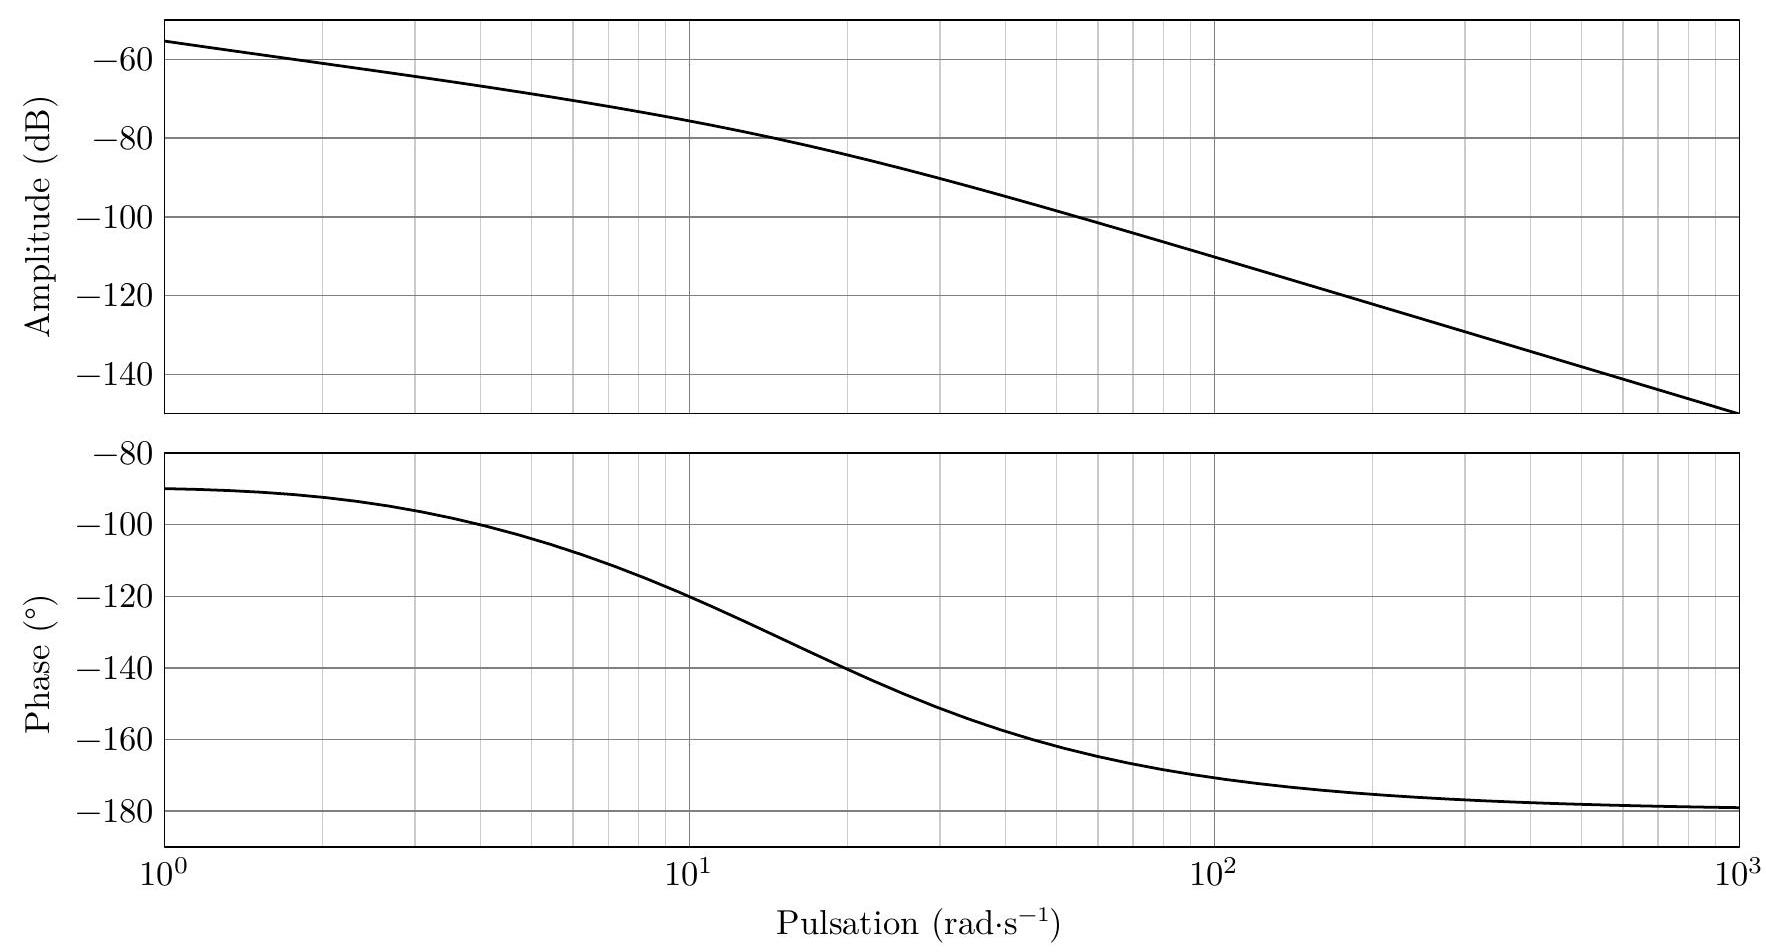
\includegraphics[width=\textwidth]{2024_03_20_0c3cf888f6e04b1986bcg-12(1)}
\caption{Diagramme de Bode de $H_{B O f}(p)$  \label{Cy_02_Ch_04_TD_02_fig_16}}
\end{figure}

\begin{marginfigure}%[!h]
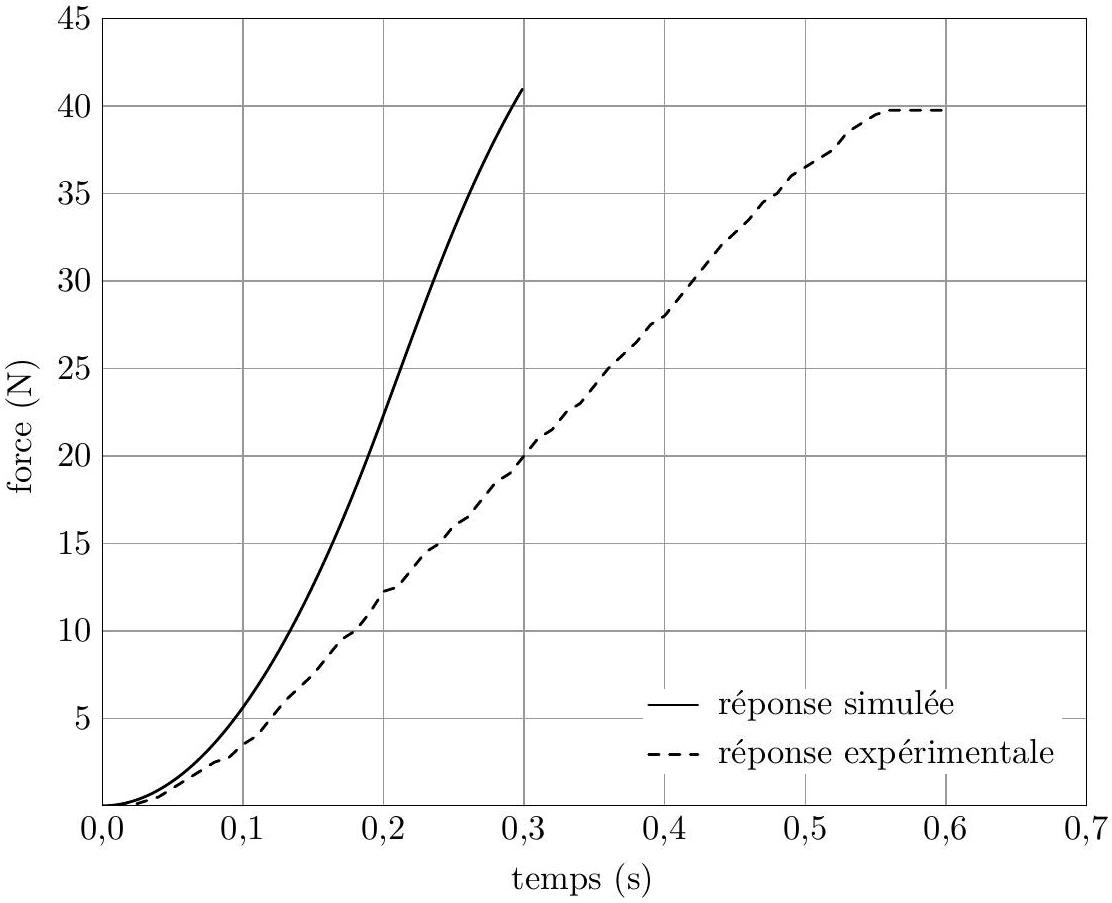
\includegraphics[width=\textwidth]{2024_03_20_0c3cf888f6e04b1986bcg-12}
\caption{Réponses temporelles du modèle et expérimentale, pour une consigne en échelon de force de $40 \mathrm{~N}$ \label{Cy_02_Ch_04_TD_02_fig_17}}
\end{marginfigure}
\fi

%Q 22
\question{Déterminer la valeur numérique limite de $K_{\text {cor }}$ afin que la boucle d'asservissement de force respecte les critères de marge de phase et de gain du tableau~\ref{Cy_02_Ch_04_TD_02_tab_05}.}
\ifprof
\begin{corrige}
La marge de gain sera toujours infinie car la phase tend asymptotiquement vers $-180\degres$.

Pour régler la marge de phase à 60\degres, il faut relever le gain de \SI{75}{dB}. On a donc $\indice{K}{cor}  =10^{75/20} \simeq  5623$.
\end{corrige}
\else
\fi



\ifprof
\else
Les courbes sur la figure \ref{Cy_02_Ch_04_TD_02_fig_17} représentent les réponses temporelles du modèle de connaissance de la figure \ref{Cy_02_Ch_04_TD_02_fig_11}, avec les correcteurs $C_{v}(p)$ et $C(p)$ correctement réglés, et de l'expérimentation sur le banc d'essai pour une consigne en échelon de force de $40 \mathrm{~N}$.
\fi


%Q 23
\question{Quel critère du tableau des exigences (tableau \ref{Cy_02_Ch_04_TD_02_tab_05}) n'est pas pris en compte dans le modèle de connaissance ? D'après la courbe expérimentale, ce critère est-il respecté par le système réel ?}
\ifprof
\begin{corrige}
La réponse temporelle du modèle ne permet pas de savoir si l'exigence 1.1 sur le dépassement est resepectée. 

Ce critère semble respecté sur le système réel vu qu'aucun dépassement n'est observé en régime permanent. 
\end{corrige}
\else
\fi

